\documentclass[11pt,a4paper]{article}

\usepackage[utf8]{inputenc}
\usepackage[T1]{fontenc}
\usepackage{lmodern}
\usepackage{microtype}
\usepackage{geometry}
\geometry{margin=2.5cm}
\usepackage{amsmath, amssymb}
\usepackage{booktabs}
\usepackage{graphicx}
\usepackage{caption}
\usepackage{xcolor}
\usepackage{hyperref}
\hypersetup{
  colorlinks   = true,
  urlcolor     = blue!60!black,
  citecolor    = blue!60!black,
  linkcolor    = blue!60!black
}
\usepackage[round,authoryear]{natbib}
\bibliographystyle{apalike}

\setlength{\parskip}{0.4em}
\setlength{\parindent}{0pt}

\title{When psychopathic traits are not traits: \\
Aggregation bias and {Big~Five} redundancy in the prediction \\
of professional success%
\thanks{\textbf{Preliminary draft v0.1, not for citation.}
Comments are welcome.}%
}

\author{%
Carlo Vilches\thanks{%
Universitat de Barcelona. Email: \texttt{cvilchce15@alumnes.ub.edu}.
Repository: \url{https://github.com/cmvdata/psychopathy-success}.%
}%
}

\date{\today}


\begin{document}
\maketitle

\begin{abstract}
\itshape
We replicate and extend \citet{eisenbarth2018}, who examine whether
psychopathic traits predict professional success on a sample of $N=439$
working adults (OSF data). The original zero-order correlation between
Fearless Dominance (FD) and Professional Satisfaction ($r=+0.13$) does
not survive once three methodological problems are addressed jointly.
First, the PPI-R total score conflates the positive effect of FD with
the negative effect of Self-Centered Impulsivity (SCI): the aggregated
correlation is $r=-0.03$, hiding an opposite-sign component structure.
Second, FD is largely captured by Big Five Extraversion and Emotional
Stability: a regression of FD on the Big Five plus demographics yields
$R^2 = 0.616$ ($N=409$), $87.5\%$ of which is recovered by Extraversion
and Emotional Stability alone; the linear ranking of predictors and the
information-theoretic ranking from the Kraskov--Stögbauer--Grassberger
(KSG) mutual information estimator agree on all five positions, and
the corrected redundancy ratio $1-I(\text{FD};\text{BF}) /
H_{\text{diff}}(\text{FD})$ equals $0.55$ --- the Big Five accounts for
$45\%$ of FD's information content, the residual $55\%$ being
idiosyncratic variance or measurement noise. Third, three causal
estimators (caliper propensity-score matching, inverse probability
weighting, and augmented IPW) applied at four treatment thresholds
(FD $>$ P50, P67, P75, P80) all return ATTs not significant at the
$5\%$ level. The caliper PSM at the median threshold drops $117$ of
$198$ treated observations ($59\%$) for lack of admissible matches
within $0.2 \cdot \text{SD}(\text{logit PS})$ --- itself a structural
symptom of redundancy: high-FD individuals have few comparable
controls because high FD is essentially high Extraversion combined
with high Emotional Stability. The methodological contribution is to
show that aggregation bias and construct redundancy jointly explain
previously reported FD effects: studies reporting an FD effect on
professional outcomes without controlling for the Big Five are likely
measuring Extraversion and Emotional Stability under a different label.
\end{abstract}

% =====================================================================
\section{Introduction}
\label{sec:intro}
% =====================================================================

\citet{eisenbarth2018} ask whether psychopathic traits, as measured
by the \citet{lilienfeld2005} Psychopathic Personality
Inventory--Revised (PPI-R), predict professional success in a sample
of working adults. They report a positive zero-order correlation
between Fearless Dominance (FD) and Professional Satisfaction
($r=0.12$, $p<0.01$ in the original) that attenuates --- but
survives --- the inclusion of Big Five controls. Their study is part
of a broader literature documenting positive associations between
``boldness'' or ``successful psychopathy'' and career outcomes, with
implications for labor economics narratives in which dominance traits
are economically rewarded.

This paper revisits the same data and finds that the FD effect on
professional success rests on three methodological foundations that
do not jointly hold.

The \emph{first} problem is aggregation bias. The PPI-R total score
sums three orthogonal dimensions: FD (positive correlate of
Professional Satisfaction in our replication, $r=+0.13$), SCI
(negative correlate, $r=-0.14$), and Coldheartedness (CO; null
correlate, $r=-0.05$). The aggregate correlation is $r=-0.03$, a
spurious null produced by the cancellation of opposite-sign component
effects. Reading the aggregated score as a meaningful construct
mistakes a measurement artefact for the absence of a relationship.

The \emph{second} problem is construct redundancy. FD is empirically
close to a linear combination of Big Five Extraversion and Emotional
Stability: the bivariate correlations are $r=+0.49$ and $r=+0.66$
respectively, and the regression $\text{FD} \sim \text{Big Five} +
\text{demographics}$ delivers $R^2 = 0.616$. A reduced model with
only Extraversion and Emotional Stability captures $87.5\%$ of that
explanatory power. A nonparametric information-theoretic check
(Kraskov--Stögbauer--Grassberger mutual information,
\citealp{kraskov2004}) confirms this: the joint mutual information
$I(\text{FD};\text{BF}_{\text{full}}) = 0.93$ bits accounts for
approximately $45\%$ of the differential entropy of FD, with
Extraversion and Emotional Stability dominating the contribution and
no detectable nonlinear residual. The linear ranking of Big Five
predictors and the information-theoretic ranking match position-by-position
($5/5$).

The \emph{third} problem is the absence of a robust causal effect.
Under three estimators (caliper propensity-score matching, inverse
probability weighting, and augmented IPW following
\citealp{robins1995}) and four candidate dichotomisations of FD
(P50, P67, P75, P80), no Average Treatment Effect on the Treated is
significant at the $5\%$ level. The caliper PSM at the median
threshold, with caliper width $0.2 \cdot \text{SD}(\text{logit PS})$
in line with the recommendation of \citet{austin2011}, drops $117$
of $198$ treated units for lack of admissible matches: the failure of
common support is itself a manifestation of redundancy, since high-FD
individuals have few control units that combine comparable
Extraversion and Emotional Stability profiles.

We make three contributions. First, a methodological diagnosis: the
three problems above are not independent. Construct redundancy
\emph{causes} the common-support failure of PSM; aggregation bias
\emph{motivates} the disaggregated analysis whose null result
triggers the redundancy diagnostic; the null causal estimates close
the loop. Second, an honest reporting of effect sizes: the
disaggregated zero-order correlations of FD and SCI with
Professional Satisfaction are non-trivial, but their predictive
$R^2$ in cross-validation is essentially zero across both linear
(OLS) and nonlinear (XGBoost) specifications. Third, a corrected
redundancy ratio for the FD--Big-Five relationship that combines
the continuous KSG mutual information with the Gaussian
differential-entropy normalisation, avoiding the unit-mismatch
that occurs when one mixes continuous mutual information with
discrete entropy of a binned variable.

The paper is organised as follows. Section~\ref{sec:data} describes
the dataset. Section~\ref{sec:method} presents the five methodological
pipelines: replication, factor structure, predictive modelling, causal
identification, and redundancy diagnostic. Section~\ref{sec:results}
reports the empirical results in the same order.
Section~\ref{sec:discussion} discusses why the three problems are
connected and what the implications are for the psychopathy and labor
literatures. Section~\ref{sec:limits} states limitations and threats
to identification. Section~\ref{sec:conclusion} concludes.

% =====================================================================
\section{Data}
\label{sec:data}
% =====================================================================

The data is the working sample from \citet{eisenbarth2018}, made
publicly available via the Open Science Framework
(\url{https://osf.io/tgujv}). It consists of self-report responses
from $N=439$ working adults after the original exclusion criteria
(failure to complete all measures, prior participation, age below 18,
non-English first language). The dataset includes:

\begin{itemize}
\item \textbf{Psychopathic traits}: the 40-item short form of the
  PPI-R \citep{lilienfeld2005}, scored into three dimensions ---
  Fearless Dominance (FD), Self-Centered Impulsivity (SCI), and
  Coldheartedness (CO) --- and a total score (PPI Total).
\item \textbf{Big Five personality}: the Ten-Item Personality
  Inventory \citep{gosling2003}, scoring Extraversion, Agreeableness,
  Conscientiousness, Emotional Stability, and Openness.
\item \textbf{Professional Satisfaction}: a composite of three
  items (Career Satisfaction, Promotion Satisfaction, Salary
  Satisfaction).
\item \textbf{Material Success}: a composite indicator combining
  professional standing, annual salary band, and promotion frequency.
\item \textbf{Demographics and controls}: age (mean $33.0$, SD
  $9.2$), gender (women $59.7\%$, men $40.3\%$), and months in current
  job.
\end{itemize}

For all analyses except those requiring complete cases on Months in
Job, the sample is $N=439$. The causal-inference and redundancy
analyses condition on $N=409$ after dropping rows with missing
covariates (most commonly Months in Job).

A caveat applies to the Material Success composite. Cronbach's
$\alpha$ is $0.48$ in the original and $0.48$ in our replication;
this is below conventional reliability thresholds for psychometric
use ($\alpha \ge 0.70$). We retain Material Success in the
descriptive analysis (Section~\ref{sec:results-replication} and
Table~\ref{tab:correlations}) for direct comparison with
\citet{eisenbarth2018} but treat Professional Satisfaction
($\alpha=0.78$) as the primary outcome for the predictive, causal,
and redundancy analyses. This reduces Section~\ref{sec:results} to a
single outcome at the cost of partial coverage of the original
research question.

% =====================================================================
\section{Methodology}
\label{sec:method}
% =====================================================================

\subsection{Replication pipeline}
\label{sec:method-replication}

We replicate the original analysis in three steps: (i) Cronbach's
$\alpha$ for the Professional Satisfaction and Material Success
composites and for PPI-R Coldheartedness \citep{cronbach1951};
(ii) zero-order Pearson correlations among PPI dimensions, Big Five
traits, and the two outcome composites (the original Table~3); and
(iii) OLS regressions of each outcome on the three PPI dimensions,
first without controls and then with Big Five and demographic
controls (the original Table~4 estimated structurally as SEM, here
estimated by OLS as a transparent approximation).

\subsection{Factor structure and aggregation diagnostic}
\label{sec:method-efa}

We perform an Exploratory Factor Analysis on the 40 PPI-R items
using oblimin rotation, after verifying sampling adequacy via
Bartlett's test of sphericity ($\chi^2 = 4{,}821.99$, $p < 0.001$)
and the Kaiser--Meyer--Olkin measure ($\text{KMO} = 0.807$, in the
``meritorious'' range). The objective is to confirm the
multidimensional structure of the inventory empirically.

The aggregation diagnostic is purely descriptive: we compute the
zero-order correlation of each PPI dimension and of the PPI Total
score with each outcome composite, and visualise the cancellation in
Figure~\ref{fig:aggregation}.

\subsection{Predictive modelling}
\label{sec:method-pred}

We compare four feature sets ---  PPI Total only; FD$+$SCI$+$CO;
FD$+$SCI$+$CO plus Big Five; full model including
demographics --- under two estimators: ordinary least squares (OLS)
and gradient-boosted trees (XGBoost) with $200$ estimators, max depth
$3$, learning rate $0.05$, and column subsampling $0.8$. The
evaluation is repeated 5-fold cross-validation with $20$ repeats
($100$ folds total), reporting cross-validated $R^2$, RMSE, and MAE.
Random states are fixed (\texttt{random\_state=42}) for
reproducibility.

\subsection{Causal identification}
\label{sec:method-causal}

The causal pipeline targets the Average Treatment Effect on the
Treated (ATT) of high Fearless Dominance on Professional Satisfaction.

\paragraph{Treatment.} The treatment indicator is
$T_i = \mathbb{1}\{\text{FD}_i > \text{P50}(\text{FD})\}$ in the main
analysis, with sensitivity at P67, P75, and P80. P50 (the median)
balances the two arms most evenly and maximises analytic power.

\paragraph{Confounders.} Eight observable confounders enter the
propensity-score model: Age, Gender (male indicator), the five Big
Five traits (Extraversion, Agreeableness, Conscientiousness,
Emotional Stability, Openness), and Months in Job. Conditional
Independence (CIA, \citealp{rosenbaum1983,imbens2015}) is assumed.

\paragraph{Propensity score.} The propensity score is estimated by
logistic regression (statsmodels \texttt{Logit}) on a design matrix
of $16$ parameters: an intercept, $8$ linear terms (the seven
continuous covariates plus the Gender indicator), and $7$ quadratic
terms for the continuous covariates only. We deliberately exclude
pairwise interactions: an earlier $19$-parameter specification with
three theoretically motivated interactions (Extraversion $\times$
Emotional Stability; Age $\times$ Months in Job; Emotional Stability
$\times$ Conscientiousness) increased McFadden pseudo-$R^2$ from
$0.447$ to $0.455$ but did not improve the bimodality of the PS
distribution; the parsimonious specification is preferred under
$N \approx 200$ treated.

\paragraph{Caliper PSM.} Following \citet{austin2011}, we match $1{:}1$
without replacement on the logit of the propensity score with caliper
$0.2 \cdot \text{SD}(\text{logit}(\hat{p}))$. Treated units with no
admissible match are dropped. Inference is via paired $t$-test
combined with a percentile bootstrap of the matched-pair differences
($B=500$); we deliberately do not re-fit and re-match the propensity
score within the bootstrap, since this is invalid for matching
estimators \citep{abadie2008}.

\paragraph{IPW.} Inverse probability weighting uses the canonical ATT
weights ($w_i = 1$ for treated, $w_i = \hat{p}_i / (1-\hat{p}_i)$ for
controls) after $p_1$/$p_{99}$ trimming of the propensity score.
Inference is by full-bootstrap with re-estimation of the propensity
score in each replicate ($B=500$).

\paragraph{Augmented IPW (AIPW).} Following the
Robins--Rotnitzky--Zhao formulation \citep{robins1995}, the ATT is
\begin{equation}
\hat{\tau}_{\text{AIPW}} = \frac{1}{n_1} \sum_{i} \left[ T_i \,
(Y_i - \hat{\mu}_0(X_i)) - (1 - T_i) \, \frac{\hat{p}_i}{1 - \hat{p}_i}
\, (Y_i - \hat{\mu}_0(X_i)) \right],
\end{equation}
where $\hat{\mu}_0(X_i)$ is an OLS prediction of the outcome on
controls. We deliberately fit $\hat{\mu}_0$ as a \emph{linear-only}
function of the eight confounders, in contrast to the $16$-parameter
propensity-score model. Specification diversity between the two
nuisance models is a precondition for the doubly-robust property: if
both models share the same nonlinear misspecification, their errors
covary and the asymptotic robustness disappears.

\paragraph{Bootstrap.} Inference for IPW and AIPW uses
$B=500$ replicates with full re-estimation of both the propensity
score and (for AIPW) the outcome model in each replicate. This
captures the joint uncertainty of the two nuisance models. Caliper
PSM uses paired-difference bootstrap on the matched sample, since
re-matching across bootstrap replicates is invalid
\citep{abadie2008}.

We report covariate balance via the Standardised Mean Difference
(SMD) before and after adjustment, with $|\text{SMD}| < 0.10$ as the
acceptable balance threshold. For caliper PSM, balance is unweighted
(matched-pair means). For IPW, balance uses the same ATT weights.
Entropy balancing \citep{hainmueller2012} is mentioned as an
alternative we did not use; we rely on the diversity of three
estimators rather than on a single best-balanced estimator.

\subsection{Construct redundancy}
\label{sec:method-redundancy}

The redundancy of FD with the Big Five is assessed in two
complementary ways.

\paragraph{Linear redundancy.} We regress FD on the Big Five and the
three demographic controls (Age, Gender, Months in Job) and report
$R^2$, adjusted $R^2$, the $F$-statistic, and standardised
coefficients. We then estimate a parsimonious reduced model with
only Extraversion and Emotional Stability and report the fraction of
the full $R^2$ recovered. Variance Inflation Factors (VIF) for the
full model assess multicollinearity among the predictors themselves
(distinct from FD's redundancy with them).

\paragraph{Information-theoretic redundancy.} We use the
Kraskov--Stögbauer--Grassberger nearest-neighbour estimator
\citep{kraskov2004} (KSG-1, $k=3$, max norm) to compute three
quantities. First, the univariate mutual information
$I(\text{FD}; \text{BF}_k)$ for each Big Five trait separately,
using the implementation in
\texttt{sklearn.feature\_selection.mutual\_info\_regression}. Second,
the joint mutual information $I(\text{FD}; \text{BF}_{\text{full}})$
between FD and the five-dimensional Big Five vector, implemented in
the script as a direct application of the KSG-1 estimator with
multivariate $Y$. Third, the incremental MI of each Big Five trait
given the other four, approximated as
$\Delta I_k = I(\text{FD};\text{BF}_{\text{full}}) -
I(\text{FD}; \text{BF}_{\text{full}\setminus\{k\}})$, which identifies
the unique contribution of each trait.

We complement these with a corrected redundancy ratio. The Shannon
entropy of FD discretised into $10$ quantile bins is
$H(\text{FD}_{\text{disc}}) \approx \log_2(10) = 3.32$ bits, but
mixing this discrete entropy with the continuous KSG mutual
information produces an inconsistent ratio. The proper redundancy
ratio uses the differential entropy of FD as the normaliser: under
the standardisation $\text{FD} \sim \mathcal{N}(0,1)$,
\begin{equation}
H_{\text{diff}}(\text{FD}) = \tfrac{1}{2} \log_2(2 \pi e) \approx
2.05 \text{ bits},
\end{equation}
and the redundancy ratio is
$1 - I(\text{FD}; \text{BF}_{\text{full}}) /
H_{\text{diff}}(\text{FD})$.

A final consistency check compares the rank-ordering of the Big Five
by univariate MI against the rank-ordering by absolute standardised
coefficient in the full OLS. Disagreement would indicate nonlinear
dependencies that the linear model does not see.

% =====================================================================
\section{Results}
\label{sec:results}
% =====================================================================

\subsection{Replication of original findings}
\label{sec:results-replication}

Table~\ref{tab:reliability} reports Cronbach's $\alpha$ for the three
constructs we replicate from the original. The values match the
\citet{eisenbarth2018} report to two decimal places. The Material
Success composite has $\alpha = 0.48$, below conventional reliability
thresholds; this is a feature of the original instrument and is
discussed in Section~\ref{sec:limits}.

\begin{table}[h!]
\centering
\caption{Internal consistency, replication of \citet{eisenbarth2018}.
Source: \texttt{output/replication\_correlation\_matrix.csv} and
console output of \texttt{scripts/01\_replication.py}.}
\label{tab:reliability}
\begin{tabular}{lcc}
\toprule
\textbf{Composite (\# items)} & $\alpha$ (this paper) & $\alpha$ (original) \\
\midrule
Professional Satisfaction (3 items) & 0.779 & 0.78 \\
Material Success (3 items)          & 0.483 & 0.48 \\
PPI-R Coldheartedness (5 items)     & 0.732 & 0.73 \\
\bottomrule
\end{tabular}
\end{table}

Table~\ref{tab:correlations} reports zero-order Pearson correlations
between PPI dimensions and the two outcome composites, alongside the
Big Five Extraversion benchmark. Three patterns appear. First, the
disaggregated PPI dimensions show opposite-sign effects on
Professional Satisfaction: FD is positively associated ($r=+0.13$),
SCI is negatively associated ($r=-0.14$), and CO is essentially
null ($r=-0.05$). Second, the PPI Total score yields $r=-0.03$ on
Professional Satisfaction (and $+0.09$ on Material Success), the
direct consequence of cancellation between FD and SCI when summed.
Third, Extraversion --- a Big Five trait, not a psychopathic trait
--- shows the largest positive correlation with both outcomes
($r=+0.14$ and $r=+0.21$), foreshadowing the redundancy diagnostic
of Section~\ref{sec:results-redundancy}.

\begin{table}[h!]
\centering
\caption{Zero-order Pearson correlations between predictors and
outcomes ($N=439$). Stars denote $p<0.05$ (*), $p<0.01$ (**),
$p<0.001$ (***). Source:
\texttt{output/replication\_correlation\_matrix.csv}.}
\label{tab:correlations}
\begin{tabular}{lcc}
\toprule
\textbf{Predictor} & \textbf{Professional Satisfaction} & \textbf{Material Success} \\
\midrule
FD              & $+0.13$**  & $+0.15$** \\
SCI             & $-0.14$**  & $-0.01$\phantom{**} \\
CO              & $-0.05$\phantom{**}  & $-0.00$\phantom{**} \\
PPI Total       & $-0.03$\phantom{**}  & $+0.09$* \\
\midrule
Extraversion    & $+0.14$**  & $+0.21$*** \\
Emotional Stab. & $+0.09$\phantom{**}  & $+0.15$** \\
\bottomrule
\end{tabular}
\end{table}

The OLS replication of the original Table~4 is consistent with the
published estimates: with Big Five and demographic controls included,
the FD coefficient on Professional Satisfaction drops from $+0.017$
($p=0.009$) to $+0.013$ ($p=0.215$), losing significance, while the
SCI coefficient remains negative and significant ($-0.023$,
$p=0.031$). For Material Success, no PPI dimension is significant
once Big Five controls are added; Extraversion is the dominant
significant predictor ($\beta=+0.086$, $p<0.001$).

\subsection{Factor structure and aggregation bias}
\label{sec:results-aggregation}

Before turning to the aggregation diagnostic, we briefly confirm the
multidimensional structure of the PPI-R that justifies disaggregation.
Bartlett's test of sphericity is highly significant
($\chi^2 = 4{,}821.99$, $p < 0.001$) and the Kaiser--Meyer--Olkin
measure ($\text{KMO} = 0.807$) is in the ``meritorious'' range,
confirming that the $40$ PPI-R items are appropriate for factor
analysis. The exploratory factor analysis with oblimin rotation
(Figure~\ref{fig:efa}) supports a multi-factor solution: the scree
plot displays a clear elbow consistent with a $2$-to-$3$ factor
structure, and the loadings heatmap shows bipolar separation between
items that load on the Fearless-Dominance factor and items that load
on the Self-Centered-Impulsivity factor. The structural premise of
the original instrument --- that the $40$ items measure orthogonal
psychological dimensions rather than a single latent psychopathy
construct --- is empirically supported.

\begin{figure}[h!]
\centering
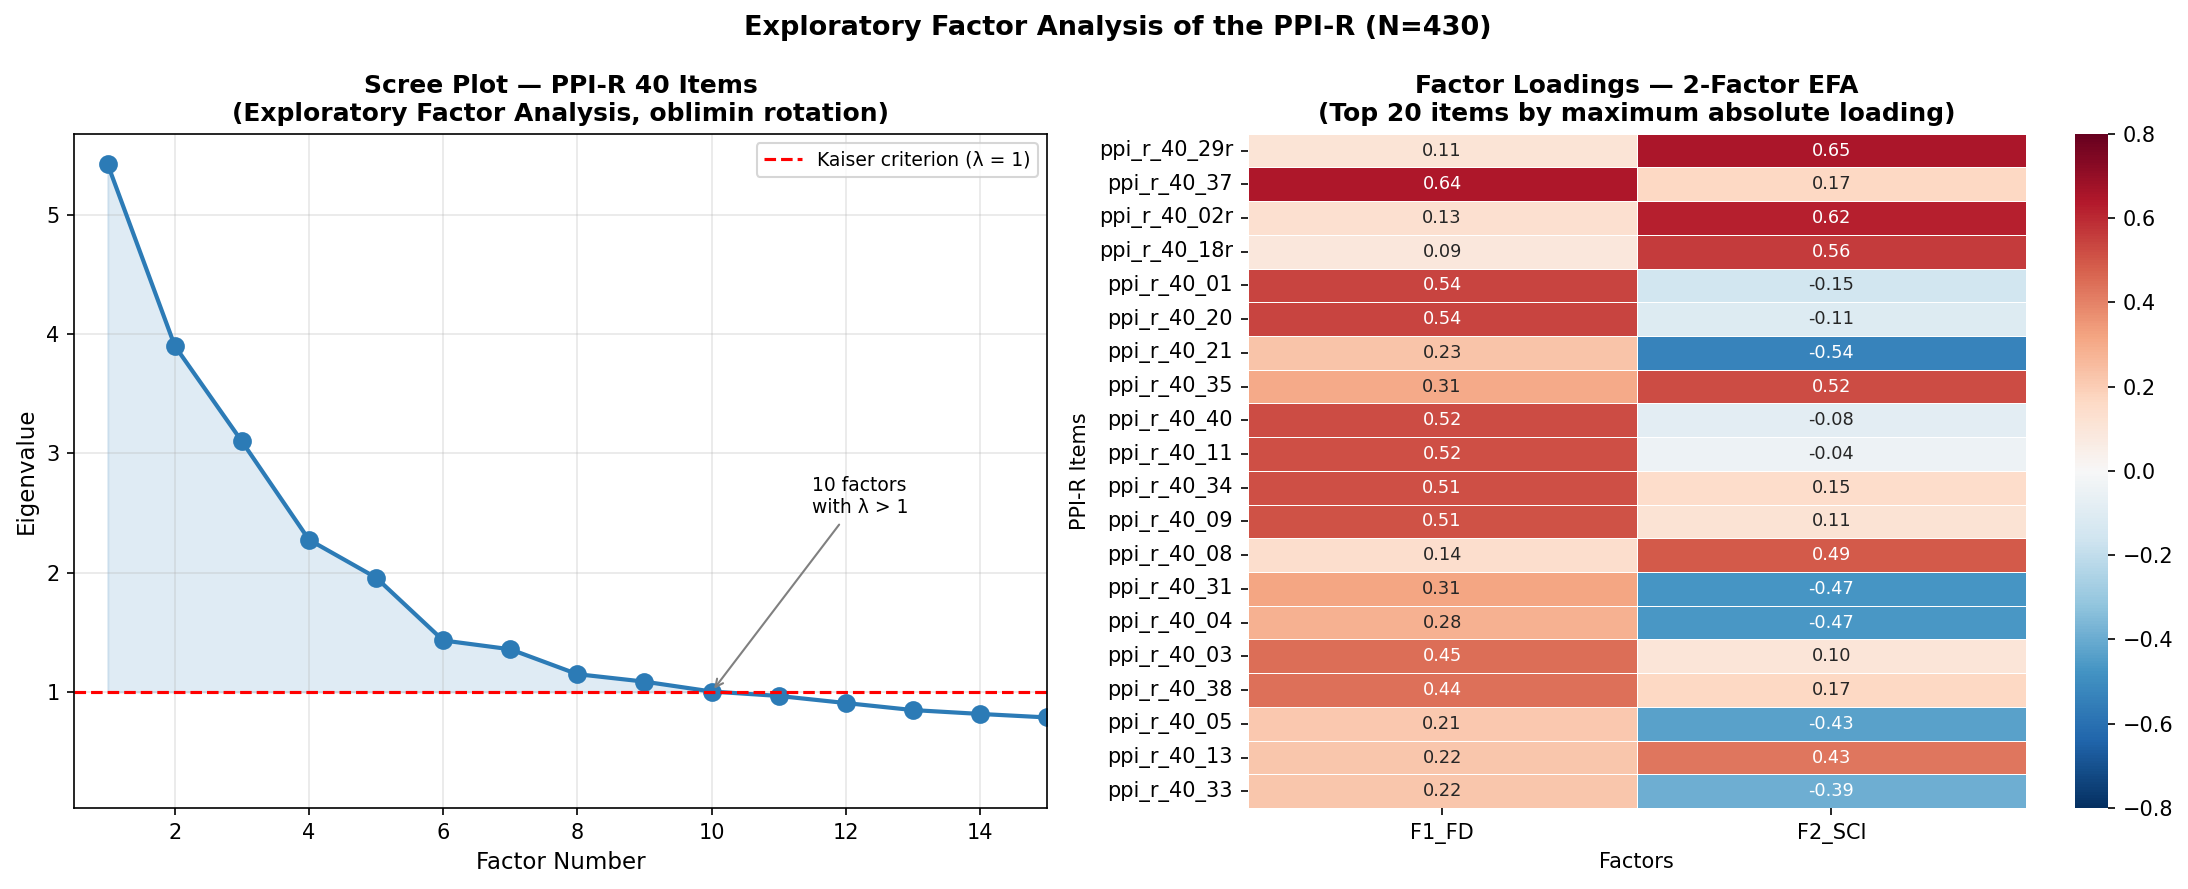
\includegraphics[width=0.85\textwidth]{../figures/fig11_efa_real.png}
\caption{Exploratory Factor Analysis of the $40$ PPI-R items
(\texttt{factor\_analyzer}, oblimin rotation, $N=430$ complete cases).
Left: scree plot with Kaiser criterion ($\lambda > 1$). Right:
$2$-factor loadings heatmap, top $20$ items by maximum absolute
loading. Source: \texttt{figures/fig11\_efa\_real.png}.}
\label{fig:efa}
\end{figure}

The aggregation bias itself is most clearly seen by visualising the
component effects against the aggregate
(Figure~\ref{fig:aggregation}). The four-panel figure confirms that
FD has a positive linear association with Professional Satisfaction,
SCI a negative one, and the PPI Total score --- being a sum of the
two oppositely-signed components plus the null CO --- yields a
near-zero slope.

\begin{figure}[h!]
\centering
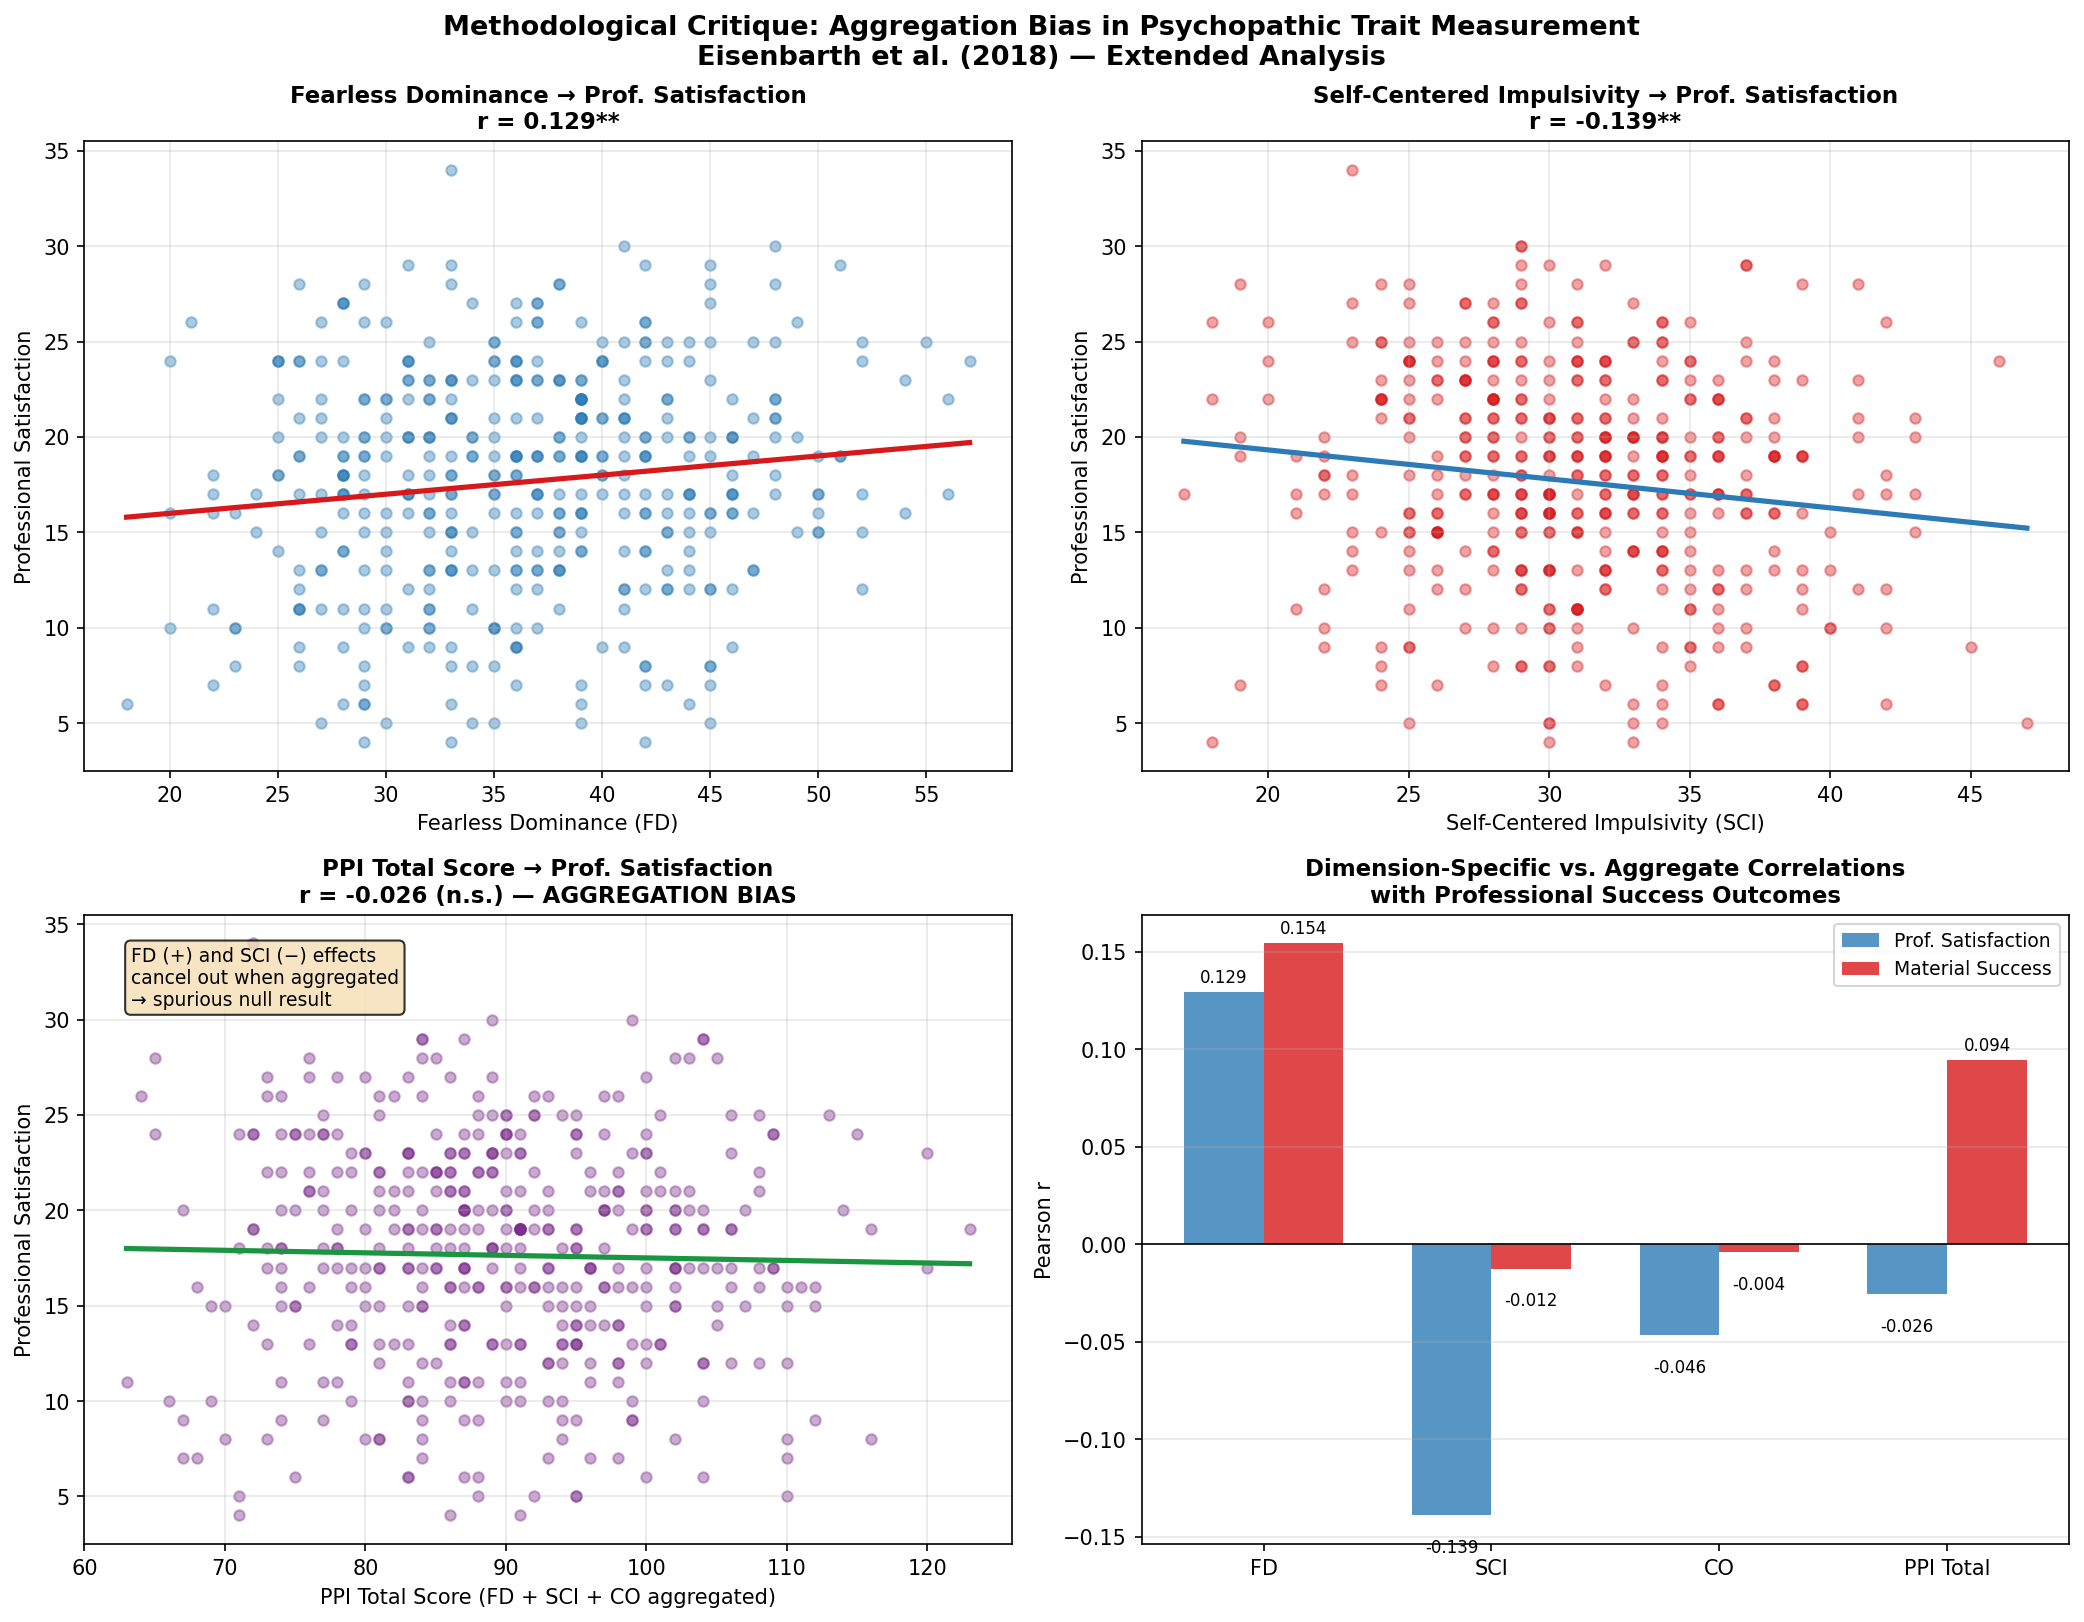
\includegraphics[width=0.85\textwidth]{../figures/fig7_aggregation_bias.png}
\caption{Aggregation bias diagnostic. Top-left: positive slope of
Professional Satisfaction on FD ($r=+0.13$). Top-right: negative slope
on SCI ($r=-0.14$). Bottom-left: near-zero slope on the PPI Total
($r=-0.03$), the cancellation of FD and SCI under aggregation.
Bottom-right: bar comparison of dimension-specific vs.\ aggregated
correlations across both outcomes. Source:
\texttt{figures/fig7\_aggregation\_bias.png} produced by
\texttt{scripts/02\_extension.py}.}
\label{fig:aggregation}
\end{figure}

\subsection{Predictive modelling}
\label{sec:results-pred}

Table~\ref{tab:cv} reports the cross-validated $R^2$ and RMSE of OLS
and XGBoost across four feature sets, on Professional Satisfaction.
The point estimate for the best-performing OLS specification (the
three PPI dimensions) is $R^2 = +0.005$; the best XGBoost
specification has $R^2 = -0.069$. All $R^2$ values are within
$\pm 0.04$ of zero or negative; none of the models predicts
Professional Satisfaction better than the unconditional mean by an
economically meaningful margin.

\begin{table}[h!]
\centering
\caption{Cross-validated predictive performance for Professional
Satisfaction (5-fold $\times$ 20 repeats; $N=439$). Source:
\texttt{output/formal\_model\_comparison.csv}.}
\label{tab:cv}
\begin{tabular}{llrrr}
\toprule
\textbf{Estimator} & \textbf{Feature set} & $\text{CV } R^2$ & $\text{CV RMSE}$ & $\text{CV MAE}$ \\
\midrule
OLS     & PPI Total only         & $-0.018$ & $5.77$ & $4.68$ \\
OLS     & FD $+$ SCI $+$ CO      & $+0.005$ & $5.70$ & $4.66$ \\
OLS     & Dimensions $+$ Big Five & $-0.011$ & $5.75$ & $4.69$ \\
OLS     & Full model              & $-0.026$ & $5.77$ & $4.75$ \\
\midrule
XGBoost & PPI Total only         & $-0.085$ & $5.95$ & $4.81$ \\
XGBoost & FD $+$ SCI $+$ CO      & $-0.069$ & $5.91$ & $4.80$ \\
XGBoost & Dimensions $+$ Big Five & $-0.073$ & $5.91$ & $4.82$ \\
XGBoost & Full model              & $-0.108$ & $6.00$ & $4.89$ \\
\bottomrule
\end{tabular}
\end{table}

Two qualitative patterns are nevertheless robust. First, separating
the three PPI dimensions yields a higher $R^2$ than aggregating them
into the PPI Total --- consistent with the aggregation-bias argument.
Second, XGBoost performs strictly worse than OLS on every feature
set, which is consistent with the absence of nonlinearities or
interactions in the underlying predictive structure: the relationship,
if any, is essentially linear and very weak.

\subsection{Causal estimates}
\label{sec:results-causal}

Table~\ref{tab:att-main} reports the main causal analysis at the
median FD threshold (P50, $N_{\text{treated}}=198$,
$N_{\text{control}}=211$, total $N=409$ after listwise deletion). The
three estimators yield positive but non-significant point estimates,
ranging from $+1.01$ (caliper PSM) to $+2.59$ (IPW). The IPW $p$-value
is marginally below the conventional $10\%$ threshold ($p=0.068$);
neither caliper PSM ($p=0.251$) nor AIPW ($p=0.147$) clears the
$10\%$ threshold.

\begin{table}[h!]
\centering
\caption{Main causal estimates at FD $>$ P50, outcome Professional
Satisfaction. The caliper PSM column reports the matched-pair sample
size; IPW and AIPW report the trimmed sample. Bootstrap with $B=500$.
Source: \texttt{output/att\_main.csv}.}
\label{tab:att-main}
\begin{tabular}{lrrrr}
\toprule
\textbf{Estimator} & \textbf{ATT} & \textbf{$95\%$ CI} & \textbf{$p$-value} & $n$ used \\
\midrule
Caliper PSM ($1{:}1$ NN, $0.2 \cdot \text{SD}(\text{logit PS})$) & $+1.012$ & $[-0.563,\,+2.674]$ & $0.251$ & $81$ pairs \\
IPW (ATT weights, $p_1/p_{99}$ trim)                              & $+2.590$ & $[-0.232,\,+5.178]$ & $0.068$ & $399$ \\
AIPW (Robins--Rotnitzky--Zhao, linear $\hat\mu_0$)                & $+2.092$ & $[-0.966,\,+5.049]$ & $0.147$ & $399$ \\
\bottomrule
\end{tabular}
\end{table}

The caliper PSM at P50 drops $117$ of $198$ treated units ($59\%$)
because no admissible control match exists within the caliper. This
is a structural symptom of the redundancy diagnosed in
Section~\ref{sec:results-redundancy}: high-FD individuals tend to be
high-Extraversion and high-Emotional-Stability simultaneously, and
the joint distribution of Big Five traits among controls does not
populate that region densely.

Figure~\ref{fig:love-caliper} reports the Love plot of standardised
mean differences before and after caliper matching at P50. Six of
the eight covariates achieve the $|\text{SMD}|<0.10$ threshold; two
do not (Extraversion, $\text{SMD}=+0.18$; Emotional Stability,
$\text{SMD}=+0.18$) --- precisely the two Big Five traits most
correlated with FD itself. The matching cannot balance covariates
that are quasi-collinear with the treatment definition.

\begin{figure}[h!]
\centering
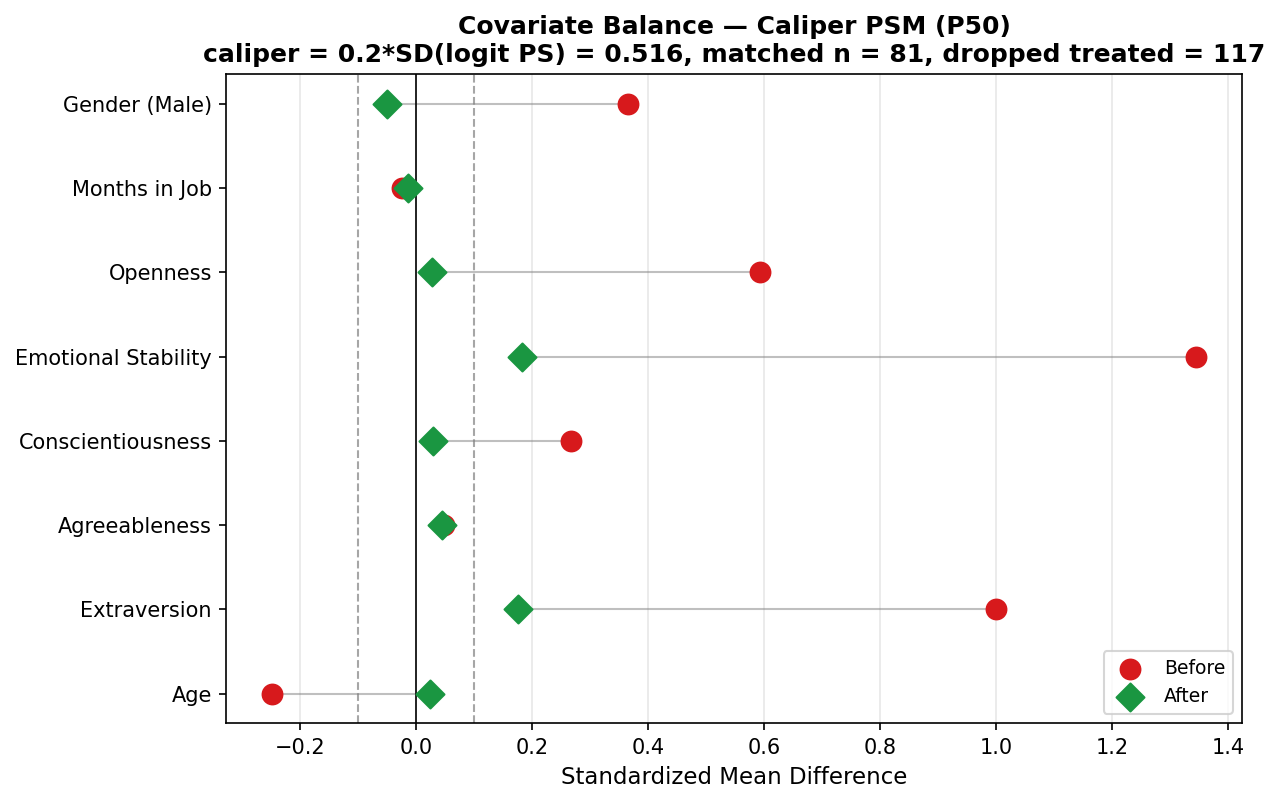
\includegraphics[width=0.85\textwidth]{../figures/love_plot_caliper.png}
\caption{Covariate balance before and after caliper PSM at FD $>$ P50.
Caliper $= 0.2 \cdot \text{SD}(\text{logit PS}) = 0.396$.
Six of eight covariates achieve $|\text{SMD}|<0.10$ (dashed lines).
Source: \texttt{figures/love\_plot\_caliper.png}.}
\label{fig:love-caliper}
\end{figure}

Figure~\ref{fig:love-ipw} shows the equivalent diagnostic for IPW.
Only Gender achieves the $|\text{SMD}|<0.10$ threshold under ATT
weights; the other seven covariates remain in the
$[0.10, 0.34]$ band of weighted SMD. The pattern is informative: the
ATT-weights re-balance the two strongest predictors of treatment
(Extraversion, Emotional Stability) at the cost of inducing weighted
imbalances in covariates with smaller marginal effects on the
propensity score (Months in Job, Agreeableness, Age). The aggregate
quality of IPW balance is therefore worse than caliper PSM by the
$|\text{SMD}|<0.10$ count (1/8 vs.\ 6/8) but with smaller maximum
magnitudes overall.

\begin{figure}[h!]
\centering
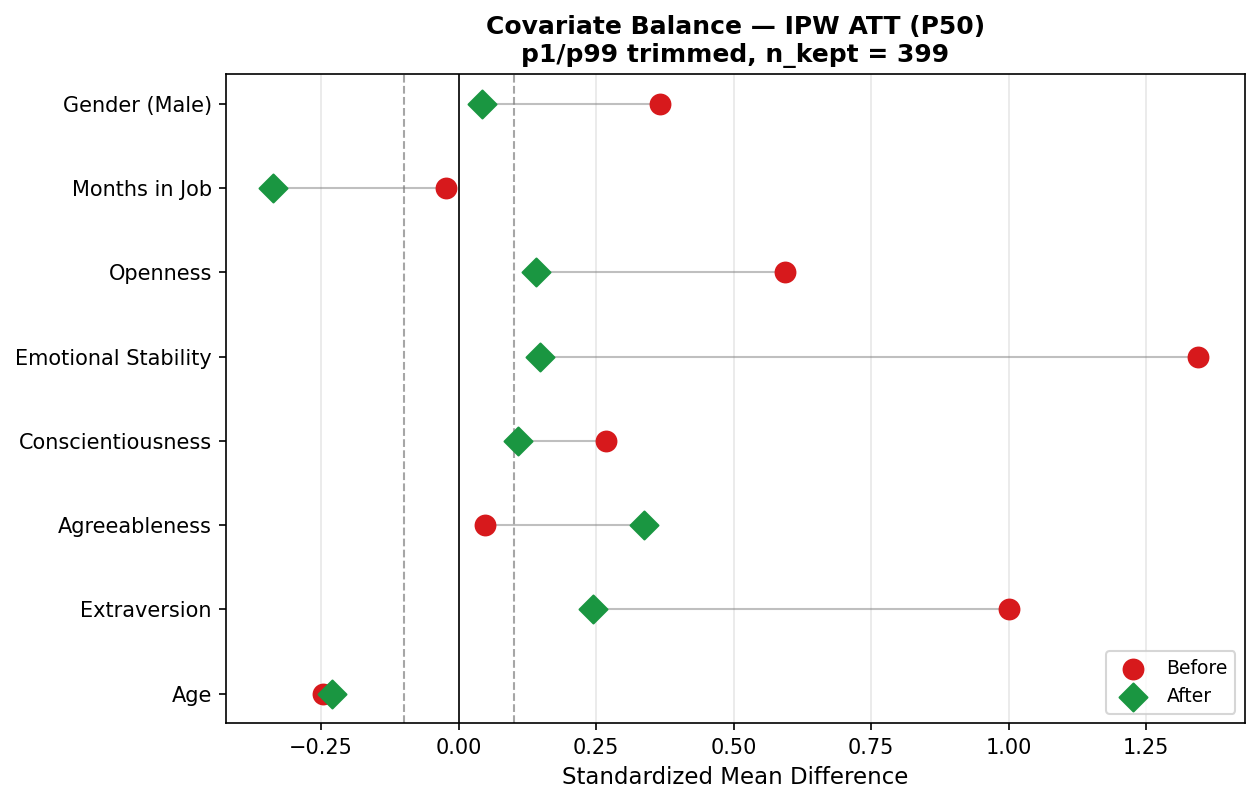
\includegraphics[width=0.85\textwidth]{../figures/love_plot_ipw.png}
\caption{Covariate balance under IPW at FD $>$ P50. ATT weights
($w=1$ for treated, $w = \hat{p}/(1-\hat{p})$ for controls) after
$p_1/p_{99}$ trimming of the propensity score. One of eight
covariates achieves $|\text{SMD}|<0.10$. Source:
\texttt{figures/love\_plot\_ipw.png}.}
\label{fig:love-ipw}
\end{figure}

Table~\ref{tab:att-sens} reports the sensitivity of the ATT to the
choice of FD threshold and estimator
(Figure~\ref{fig:sensitivity-forest} visualises this). No
combination of threshold and estimator produces an ATT significant
at the $5\%$ level; the IPW $p=0.068$ at P50 is the lowest. Across
thresholds, the sign of the ATT switches between estimators and is
not monotonic: the highest-FD subgroup (P80, $n_{\text{treated}}=77$)
yields an ATT close to zero ($+0.09$ AIPW, $+0.14$ IPW, $+1.23$
caliper PSM), the opposite of what one would expect under a
genuine FD effect compounding with the strength of the treatment.

\begin{table}[h!]
\centering
\caption{Sensitivity of ATT to FD threshold across the three
estimators. Bootstrap $95\%$ CIs in brackets. Source:
\texttt{output/att\_sensitivity.csv}.}
\label{tab:att-sens}
\begin{tabular}{lrrr}
\toprule
\textbf{Threshold} & \textbf{Caliper PSM} & \textbf{IPW} & \textbf{AIPW} \\
\midrule
P50 ($n_t=198$) & $+1.01\,[-0.56,\,+2.67]$ & $+2.59\,[-0.23,\,+5.18]$ & $+2.09\,[-0.97,\,+5.05]$ \\
P67 ($n_t=135$) & $-0.70\,[-2.42,\,+1.03]$ & $-0.19\,[-2.28,\,+3.04]$ & $-0.19\,[-3.10,\,+4.69]$ \\
P75 ($n_t= 88$) & $+0.55\,[-1.40,\,+2.75]$ & $-0.13\,[-1.99,\,+2.08]$ & $-0.15\,[-2.34,\,+2.92]$ \\
P80 ($n_t= 77$) & $+1.23\,[-0.59,\,+3.08]$ & $+0.14\,[-1.54,\,+2.22]$ & $+0.09\,[-1.58,\,+2.54]$ \\
\bottomrule
\end{tabular}
\end{table}

\begin{figure}[h!]
\centering
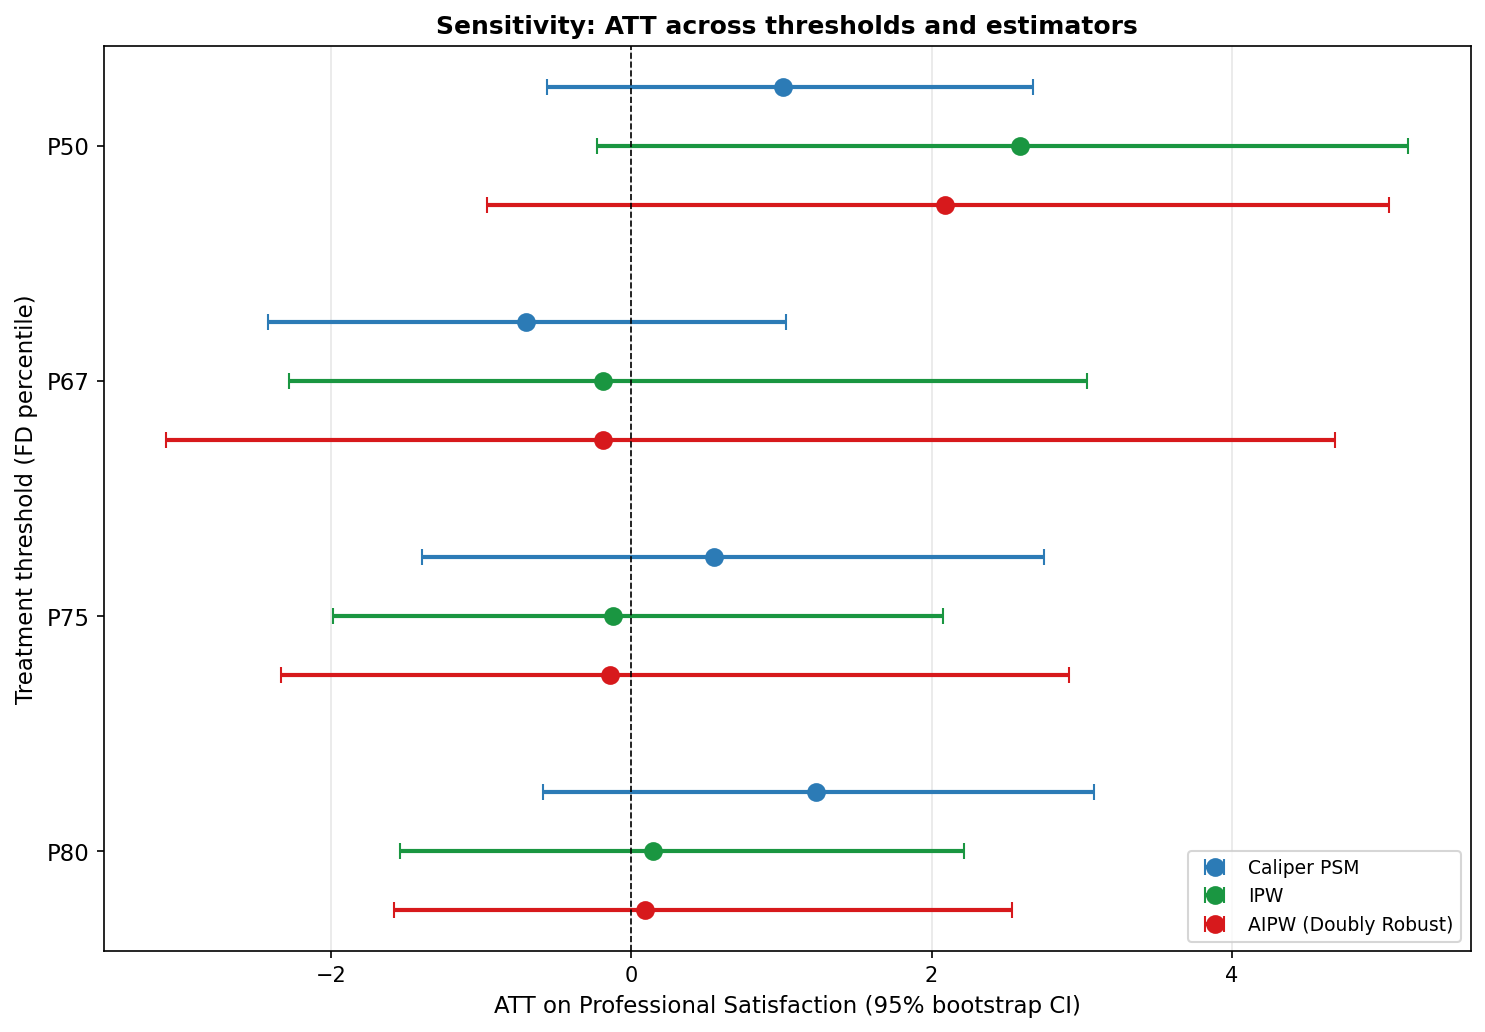
\includegraphics[width=0.85\textwidth]{../figures/sensitivity_forest_plot.png}
\caption{Sensitivity of the ATT across four thresholds and three
estimators, with $95\%$ bootstrap CIs ($B=500$, full propensity-score
re-fit per replicate for IPW and AIPW; matched-pair bootstrap for
caliper PSM). Source: \texttt{figures/sensitivity\_forest\_plot.png}.}
\label{fig:sensitivity-forest}
\end{figure}

\subsection{Construct redundancy}
\label{sec:results-redundancy}

Table~\ref{tab:redundancy} reports the linear and information-theoretic
redundancy diagnostics. Panel~A shows that the regression of FD on
the Big Five plus Age, Gender, and Months in Job yields $R^2=0.616$
($N=409$, $F=80.11$, $p < 10^{-77}$). The reduced model with only
Extraversion and Emotional Stability captures $R^2=0.539$, or
$87.5\%$ of the full-model explanatory power. The standardised
coefficients confirm that Emotional Stability ($\beta=+0.51$,
$p < 10^{-36}$) and Extraversion ($\beta=+0.30$, $p < 10^{-16}$) are
the dominant predictors of FD; Agreeableness and Conscientiousness
are not significant. VIF among the predictors themselves are all
below $1.5$, indicating that the redundancy is between FD and the
joint Big Five vector, not multicollinearity within the Big Five.

Panel~B reports the information-theoretic counterpart. Univariate
mutual information confirms the linear pattern: Emotional Stability
contributes $0.47$ bits, Extraversion $0.17$ bits; the remaining
three Big Five traits contribute essentially zero. The joint MI of
FD with the five-dimensional Big Five vector is $0.93$ bits. The
incremental MI of each Big Five given the other four is positive
only for Emotional Stability ($+0.27$ bits) --- the other four show
zero or negative incremental contribution due to KSG estimator
variance at $N=409$, but the qualitative point is unambiguous: only
Emotional Stability adds unique information once the others are
known. The differential entropy of standardised FD is
$H_{\text{diff}}(\text{FD}) = \tfrac{1}{2}\log_2(2\pi e) = 2.05$
bits; the corrected redundancy ratio is
$1 - 0.93/2.05 = 0.55$. The Big Five jointly accounts for $45\%$ of
FD's information content; the remaining $55\%$ is idiosyncratic
variance or measurement noise, with no detectable structure given
the Big Five.

The rank-ordering of the Big Five by univariate MI (Emotional
Stability, Extraversion, Openness, Conscientiousness, Agreeableness)
matches the rank-ordering by absolute standardised coefficient
\emph{position by position} ($5/5$). This is direct evidence that
the FD--Big-Five relationship is well-described by a linear model:
the information-theoretic estimator does not reveal any nonlinear
structure that the OLS would miss.

\begin{table}[h!]
\centering
\caption{Construct redundancy of FD with Big Five. Panel~A: linear
diagnostics ($N=409$). Panel~B: information-theoretic diagnostics
(KSG-1, $k=3$). Sources:
\texttt{output/fd\_redundancy\_analysis.csv} and
\texttt{output/fd\_redundancy\_information.csv}.}
\label{tab:redundancy}
\begin{tabular}{lr}
\toprule
\multicolumn{2}{l}{\textbf{Panel~A: Linear redundancy}} \\
\midrule
OLS full $R^2$ (FD $\sim$ Big Five $+$ Age $+$ Gender $+$ Months in Job) & $0.616$ \\
OLS reduced $R^2$ (FD $\sim$ Extraversion $+$ Emotional Stability)        & $0.539$ \\
Reduced fraction of full $R^2$                                            & $87.5\%$ \\
$F$-statistic (full model)                                                & $80.11$ ($p<10^{-77}$) \\
Pearson $r$ (FD, Emotional Stability)                                     & $+0.66$*** \\
Pearson $r$ (FD, Extraversion)                                            & $+0.49$*** \\
Standardised $\beta$ on Emotional Stability                               & $+0.51$ ($p<10^{-36}$) \\
Standardised $\beta$ on Extraversion                                      & $+0.30$ ($p<10^{-16}$) \\
Maximum VIF among Big Five (no multicollinearity within BF)               & $1.39$ \\
\midrule
\multicolumn{2}{l}{\textbf{Panel~B: Information-theoretic redundancy (bits)}} \\
\midrule
$H_{\text{diff}}(\text{FD})$ (Gaussian, $\sigma=1$): $\tfrac{1}{2}\log_2(2\pi e)$ & $2.05$ \\
Joint MI $I(\text{FD}; \text{BF}_{\text{full}})$ (KSG-1)                          & $0.93$ \\
Univariate MI: Emotional Stability                                                & $0.47$ \\
Univariate MI: Extraversion                                                       & $0.17$ \\
Univariate MI: Openness                                                           & $0.15$ \\
Univariate MI: Conscientiousness                                                  & $0.06$ \\
Univariate MI: Agreeableness                                                      & $0.00$ \\
Incremental MI of Emotional Stability (given other 4 BFs)                         & $0.27$ \\
Redundancy ratio $1 - I(\text{FD}; \text{BF}) / H_{\text{diff}}(\text{FD})$       & $0.55$ \\
MI ranking vs.\ $|\beta|$ ranking agreement                                       & $5/5$ \\
\bottomrule
\end{tabular}
\end{table}

% =====================================================================
\section{Discussion}
\label{sec:discussion}
% =====================================================================

\subsection{Why the three problems are connected}

The three problems we diagnose --- aggregation bias, construct
redundancy, and null causal effect --- are not independent. They
share a common architecture.

Aggregation bias is the symptom that motivates the rest. The PPI Total
yields a near-zero correlation with Professional Satisfaction
($r=-0.03$), which would lead a naive analyst either to dismiss the
psychopathy--success question or to seek nonlinearities. We instead
disaggregate, recovering FD's positive correlation ($r=+0.13$) and
SCI's negative correlation ($r=-0.14$). At this point a typical
empirical paper would report the FD effect on Professional
Satisfaction and stop.

The redundancy diagnostic intervenes here. Once we observe that
$R^2(\text{FD} \sim \text{Big Five}) = 0.62$, with Extraversion and
Emotional Stability accounting for $87.5\%$ of that --- and the
information-theoretic check confirming the linear pattern --- the
question of FD's incremental causal contribution becomes substantively
unanswerable from observational data: the construct of interest is
near-linear in the controls. This is precisely what we observe in
the causal pipeline. The caliper PSM at P50 drops $59\%$ of treated
units because the treatment region has no comparable control region
in the joint Big Five space; the IPW weights re-balance the two
strongest predictors at the cost of imbalance on others; the AIPW
estimator splits the difference between the two and yields a wider
confidence interval. None of the estimators identifies a
significant ATT.

The honest reading is therefore not ``FD has no causal effect'' in
the strong sense --- the data do not allow that strong inference.
The honest reading is that the research design is uninformative for
the FD effect because the treatment is too close to a deterministic
function of the controls.

\subsection{Implications for the psychopathy literature}

A non-trivial fraction of empirical work in personality psychology
and labor economics reports associations between PPI Total or FD and
career outcomes without controlling for Big Five Extraversion and
Emotional Stability. Our diagnostic suggests that any such association
is likely to disappear or diminish substantially once the Big Five
controls are included. This is not a novel observation in
personality theory --- \citet{miller2012} have argued the redundancy
case for the PPI's lower-order factors --- but the joint diagnostic
combining linear regression and KSG mutual information is, to our
knowledge, new for this dataset. The practical recommendation is that
PPI Total or FD should not be reported as a predictor of professional
outcomes without an explicit Big Five control specification, and that
the reduction of the FD coefficient when Big Five controls are added
is a structural feature of the construct, not a confound to be
explained away.

The Triarchic conceptualisation of psychopathy
\citep{patrick2009}, which decomposes psychopathy into Boldness,
Meanness, and Disinhibition, partly anticipates this concern: the
``Boldness'' factor is widely understood to overlap heavily with
adaptive personality traits (Extraversion, low Neuroticism), and our
findings reinforce that overlap empirically.

\subsection{Implications for labor economics}

The labor-economics literature on non-cognitive skills, surveyed by
\citet{borghans2008} and consolidated by \citet{heckman2012},
establishes that personality traits predict earnings, employment,
and occupational attainment at magnitudes quantitatively comparable
to cognitive ability for many outcomes, and that ignoring them
generates omitted-variable bias in returns-to-schooling estimates.
Within this literature the Big Five is the canonical
operationalisation. \citet{mueller2006}, using longitudinal earnings
data, estimate non-trivial returns to one standard deviation of each
Big Five trait, with substantial gender heterogeneity in which traits
carry the strongest returns. Against this baseline, any claim that a
distinct ``psychopathy premium'' exists in professional outcomes is
implicitly a claim that some FD-related trait variation remains
\emph{after} conditioning on the Big Five and contributes
independently to compensation or satisfaction. The empirical bar is
therefore not whether FD correlates with success in raw data ---
\citet{eisenbarth2018} confirm it does --- but whether FD adds
information that the Big Five does not already carry.

The diagnostic of Section~\ref{sec:results-redundancy} answers this
question negatively in the present data. FD is not statistically
separable from Extraversion combined with Emotional Stability: the
linear $R^2$ of FD on the Big Five and demographics is $0.62$, the
corrected redundancy ratio $1 - I/H_{\text{diff}}$ is $0.55$, and
the rank-orderings produced by the linear model and by the KSG
mutual-information estimator agree on all five Big Five positions.
A premium attributable to FD, in this sample, collapses mechanically
into the premium already documented by the Big Five literature for
Extraversion and Emotional Stability. There is no residual variation
in FD --- after conditioning on the Big Five --- that could be
reassigned to a distinct ``successful psychopathy'' construct.

The policy implication of this redundancy depends on which narrative
one accepts. The first narrative, ``psychopathy is rewarded in the
workplace'', treats FD as a distinct trait cluster of dark
personality features that labour markets have mis-priced, and
suggests a policy response of re-designing hiring and promotion
processes to penalise it. The second narrative, ``social confidence
and emotional resilience are rewarded'', treats the same statistical
pattern as the conventional return to non-pathological personality
already documented in the Big Five literature
\citep{borghans2008,mueller2006}, and suggests the more conventional
policy implication of recognising personality as a labor-market input
alongside cognitive ability and human capital. Our null causal
results, conditional on the redundancy, suggest the second narrative
is the more parsimonious description of the data.

% =====================================================================
\section{Limitations and threats to identification}
\label{sec:limits}
% =====================================================================

This is a working draft (v0.1). Several limitations apply.

\textbf{Material Success reliability.} The Material Success
composite has Cronbach's $\alpha = 0.48$, well below conventional
psychometric thresholds. We retain Material Success only for the
descriptive replication (Table~\ref{tab:correlations}); the predictive,
causal, and redundancy analyses use Professional Satisfaction
($\alpha=0.78$) as the primary outcome. This restricts the scope of
the conclusions to Professional Satisfaction and leaves Material
Success unaddressed by our extension.

\textbf{Predictive performance is near zero.} The cross-validated
$R^2$ of every model in Table~\ref{tab:cv} is within a few percent
of zero or negative. This is a substantive limit: even if the FD
effect were real, no model in our specification space predicts
Professional Satisfaction well from any combination of psychopathic
traits, Big Five traits, and demographics. The variance explained by
all available predictors is small relative to the residual.

\textbf{Conditional Independence Assumption.} Identification of the
ATT requires that, conditional on the eight observed covariates,
treatment assignment is independent of potential outcomes. We do not
observe cognitive ability, socioeconomic background, sectoral
heterogeneity, or industry-specific compensation structures. Any of
these may correlate with both self-rated FD and professional success,
violating CIA in directions we cannot bound.

\textbf{Reverse causality.} Professional success may causally
elevate self-reported Fearless Dominance over time. The PPI-R is
self-administered at a single time point; we cannot separate
``confident successful person'' from ``successful person who
became more confident as a consequence of success.''

\textbf{Self-report measurement error.} Both the predictors (PPI-R,
Big Five) and one of the outcomes (Professional Satisfaction) are
self-reported. Self-rating bias may inflate the apparent correlation
between personality and self-perceived success. The Material Success
composite is partially anchored on objective indicators (annual
salary band, promotion frequency) but its reliability is low.

\textbf{Non-experimental treatment.} The treatment ``high FD'' is
defined by thresholding a continuous personality measure. This is
not a treatment in the experimental sense; the comparison group is a
post-hoc partition of the same population on a self-reported trait
that, as Section~\ref{sec:results-redundancy} establishes, is
near-linear in the Big Five controls.

\textbf{Common-support failure.} The caliper PSM drops $59\%$ of
treated units at P50. The reported caliper-PSM ATT is therefore
restricted to the $81$ treated units who do find an admissible
match; the $117$ units without a match represent a region of the
covariate space where causal inference under CIA is not feasible
from this sample.

% =====================================================================
\section{Conclusions}
\label{sec:conclusion}
% =====================================================================

Three convergent lines of evidence support the view that Fearless
Dominance is not empirically separable from Big Five Extraversion and
Emotional Stability in this sample. First, the original PPI Total
correlation with Professional Satisfaction ($r=-0.03$) is a spurious
null produced by the cancellation of opposite-sign FD ($+0.13$) and
SCI ($-0.14$) component effects. Second, FD is captured at $R^2=0.62$
by the Big Five plus demographics, with $87.5\%$ of that recovered by
Extraversion and Emotional Stability alone, and the
information-theoretic redundancy ratio is $0.55$ --- of FD's
information content, $45\%$ is shared with the Big Five and the
remainder is idiosyncratic. Third, three causal estimators applied at
four FD thresholds yield no ATT significant at $5\%$, and the caliper
PSM at the median threshold drops $59\%$ of treated units for lack of
admissible matches.

The contribution is methodological. The combination of (i) an
aggregation-bias diagnostic, (ii) a corrected redundancy ratio that
combines the KSG mutual information with Gaussian differential
entropy, and (iii) a causal pipeline with three estimators and four
thresholds gives a transparent template for assessing whether a
candidate construct adds incremental information to a baseline of
established personality dimensions. Applied here, the template
suggests that previously reported FD effects on professional outcomes
are plausibly attributable to the Big Five components on which FD
loads.

Future work suggested by this analysis includes longitudinal designs
to address reverse causality directly --- the available cross-section
cannot --- and instrumental-variable strategies for FD that exclude
the Big Five from the first stage. Both are demanding empirical
projects given the apparent linearity of FD in the Big Five; the
exclusion restriction in particular requires a source of variation in
FD that is plausibly orthogonal to Extraversion and Emotional
Stability, which is not obviously available in standard personality
datasets. A complementary direction is the application of the same
three-pronged diagnostic to other ``successful psychopathy''
operationalisations in labour-economics datasets, to assess whether
the redundancy with Big Five generalises beyond the PPI-R.

% =====================================================================
\bibliography{refs}
% =====================================================================

\end{document}
